\section{Determination of $\rho$}
\label{sec:rho}

%----------------------------------------------------------------------------------------------------
\subsection{Coulomb-Nuclear Interference}
\label{sec:rho cni}

\TODO{Summarise the theoretical models we use. A shorter version of what we had in 1km with references to that paper.}

%----------------------------------------------------------------------------------------------------
\subsection{Data fits}
\label{sec:rho anal}

\TODO{Analysis procedure}

\TODO{Our best fit}

\TODO{Fit most fair for comparison with previous measurements}

\begin{figure*}
\vskip-5mm
\begin{center}
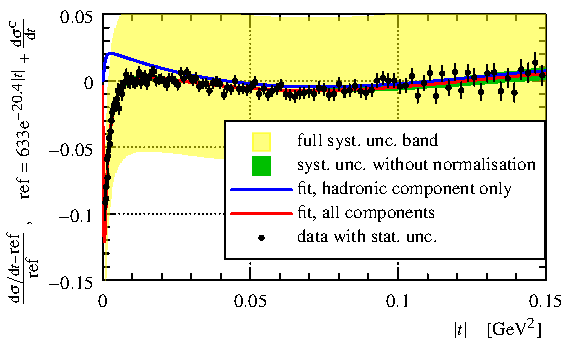
\includegraphics{fig/fit_details_exp3_0p15.pdf}
\caption{%
fit exp3, tmax 0.15,
\TODO{describe},
\TODO{add systematics to plots}
}
\label{fig:fit exp3 0.15}
\end{center}
\end{figure*}


\begin{figure*}
\vskip-5mm
\begin{center}
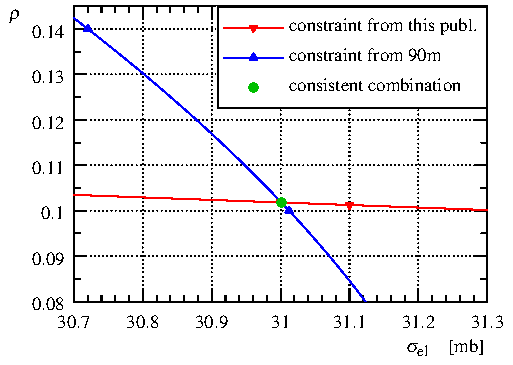
\includegraphics{fig/si_el_rho_solution.pdf}
\caption{%
\TODO{describe},
}
\label{fig:si_el rho sol}
\end{center}
\end{figure*}





\begin{figure*}
\vskip-5mm
\begin{center}
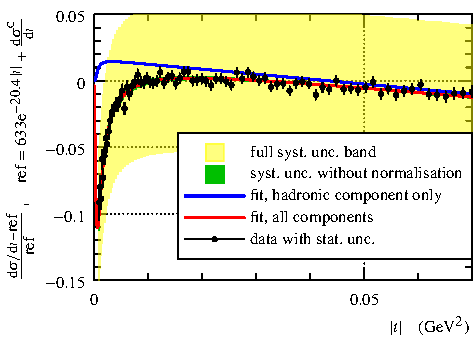
\includegraphics{fig/fit_details_exp1_0p07.pdf}
\caption{%
fit exp1, tmax 0.07,
\TODO{describe},
\TODO{add systematics to plots}
}
\label{fig:fit exp1 0.07}
\end{center}
\end{figure*}




\begin{figure*}
\vskip-5mm
\begin{center}
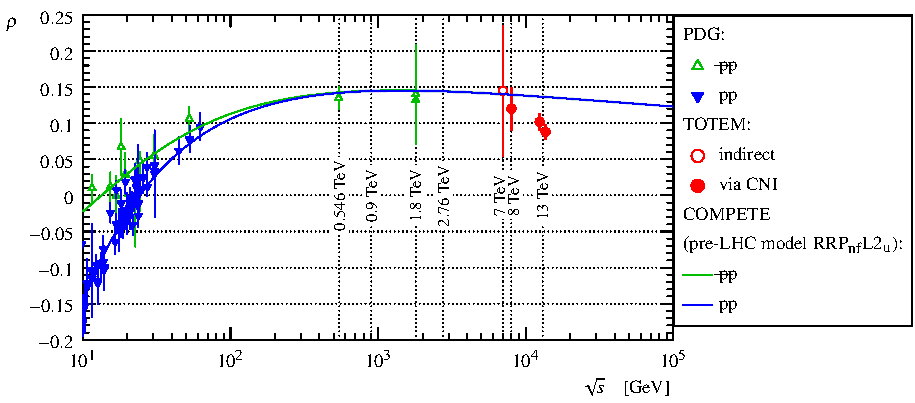
\includegraphics{fig/rho_vs_s.pdf}
\caption{%
\TODO{write}
}
\label{fig:rho_vs_s}
\end{center}
\end{figure*}
